

\newcommand{\largo}{\text{la}}
\newcommand{\nsf}{\text{nsf}}

\textbf{Advertencia.} Para evitar confusiones, en esta pregunta considere el uso de paréntesis visto en la clase 0, es decir, no elimine paréntesis innecesarios.\medskip

En clases definimos de informalmente el árbol sintáctico de una fórmula proposicional $\varphi$ como aquel tal que
\begin{itemize}
	\item su raíz es $\varphi$
	\item cada nodo tiene como hijos a sus subfórmulas inmediatas
	\item cada hoja es una variable proposicional
\end{itemize}
con la posibilidad de que existan nodos repetidos. Se define el número de subfórmulas de $\varphi$ como el número de nodos en su árbol sintáctico.
Por ejemplo, para $((\neg(\neg p))\leftrightarrow ((\neg p)\wedge q))$, el número de subfórmulas es 8, dado que su árbol sintáctico es 

\begin{center}
	\newcommand\nd{15mm}
	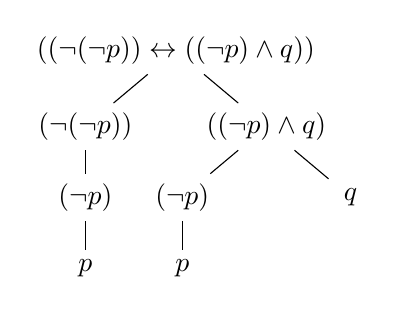
\begin{tikzpicture}[
			vertex/.style={draw=none,rectangle,minimum width=7mm},
			% node distance=10mm,
			scale=1, every node/.style={scale=1}
		]
		\node [vertex] (v0) {$((\neg(\neg p))\leftrightarrow ((\neg p)\wedge q))$};
		% \node [vertex,label=above:{$-1$}] (v0) {$H$};
		\node [vertex] (v1) at ([shift=({220:1*\nd})]v0)  {$(\neg(\neg p))$};
		\node [vertex] (v2) at ([shift=({320:1*\nd})]v0)  {$((\neg p)\wedge q)$};

		\node [vertex] (v3) at ([shift=({270:0.6*\nd})]v1)  {$(\neg p)$};
		\node [vertex] (v4) at ([shift=({270:0.6*\nd})]v3)  {$p$};

		\node [vertex] (v5) at ([shift=({220:0.93*\nd})]v2)  {$(\neg p)$};
		\node [vertex] (v6) at ([shift=({320:0.93*\nd})]v2)  {$q$};


		\node [vertex] (v7) at ([shift=({270:0.6*\nd})]v5)  {$p$};

		
		\draw[] (v0)--(v1);
		\draw[] (v0)--(v2);
		\draw[] (v1)--(v3);
		\draw[] (v3)--(v4);
		\draw[] (v2)--(v5);
		\draw[] (v2)--(v6);
		\draw[] (v5)--(v7);
	\end{tikzpicture}
\end{center}


\begin{enumerate}[label=(\alph*)]

	\item Defina de manera inductiva la función $\nsf(\varphi)$ que retorna la cantidad de subfórmulas de $\varphi$.  Por ejemplo, $\nsf(((p \vee q) \to (p \wedge (\neg r)))) = 8$.

	\item Defina $\largo(\alpha)$ como el largo de la fórmula proposicional $\alpha$, que cuenta cada símbolo y variable mencionado en $\alpha$. Por ejemplo, $\largo(((p \vee q) \to (p \wedge (\neg r))))=16$.
    
    \item Demuestre que para toda fórmula $\varphi$ se tiene que $\nsf(\varphi) \leq \largo(\varphi)$. 
\end{enumerate}